\documentclass[screen, aspectratio=43]{beamer}
\usepackage[T1]{fontenc}
\usepackage[utf8]{inputenc}

% Use the NTNU-temaet for beamer 
% \usetheme[style=ntnu|simple|vertical|horizontal, 
%     language=bm|nn|en, 
%     smalltitle, 
%     city=all|trondheim|alesund|gjovik]{ntnu2017}
\usetheme[style=ntnu,language=en]{ntnu2017}

\usepackage[english]{babel}
\usepackage[style=numeric,backend=biber,natbib=false,sorting=none]{biblatex}
\usepackage{xcolor}

\title[AP-intro]{MCT4048: Audio Programming}
\subtitle{The Fundamentals: Sound Effects}
\author[A. Xamb{\'o}]{Anna Xamb{\'o}}
\institute[NTNU]{Department of Music, NTNU}
\date{7 February 2019}
%\date{} % To have an empty date

\addbibresource{../ap.bib} % Add bibliography database

% Set the reference style to numeric.
% See here: http://tex.stackexchange.com/questions/68080/beamer-bibliography-icon
\setbeamertemplate{bibliography item}[text] 

% Set bibliography fonts to a small size.
\renewcommand*{\bibfont}{\footnotesize}

\begin{document}

\begin{frame}
  \titlepage
\end{frame}

% Alternatively, special title page command to get a different background
% \ntnutitlepage

%
\begin{frame}
\frametitle{Assignment 1: Presentation WAC paper (individual)}

Present a summary of a WAC paper of your choice to the class.\\ 
The presentation should last 5 min + 1 min for questions.

\vspace{10 mm}

Schedule of presentations 7.2.19:
\begin{itemize}
\item Ashane
\item Eigil
\item Eirik
\item Guy
\item Jonas
\item Jørgen
\end{itemize}
\end{frame}
%
\begin{frame}
\frametitle{This Week: The Fundamentals (40\% Individual Work)}
\begin{itemize}
\item \textbf{Syllabus}: \url{https://uio.instructure.com/courses/17406}
\item \textbf{Assignment 1} (Total grade: 10\%): Presentation WAC paper (individual) -- \textbf{\textcolor{olive}{day 3 (February 7, 2019)}} or 4 (February 8, 2019)
\item \textbf{Assignment 2} (Total grade: 20\%): Presentation mini-project 1 (individual) -- \textcolor{olive}{days 2 (February 6, 2019) (5\%)}, \textbf{\textcolor{olive}{3 (February 7, 2019) (5\%)}}, 4 (February 8, 2019) (10\%)
\item \textbf{Assignment 3} (Total grade: 10\%): Written blog post about the mini-project 1 -- February 11, 2019
\end{itemize}
\end{frame}
%
\begin{frame}
\frametitle{Program: Day 3 -- 7 February, 2019}
\begin{itemize}
\item 9.15-10.30: WAC paper presentations (1/2)
\item 10.30-11.00: Setting up computers with the tools for the tutorial
\item 11.00-12.30: Tutorial: Dealing with sound effects
\item 12.30-13.00: Lunch break
\item 13:00-15:00: Mini-project 1 development (3/4)
\item 15.00-16.00: Speedy presentations mini-project 1 (2/3)
\end{itemize}
\end{frame}
%
\begin{frame}
\frametitle{Learning Outcomes}
\begin{itemize}
\item Get a sense of the available effects in Web Audio.
\item Get familiar with how the effects nodes can be incorporated in the node graph.
\item Be able to create an independent project relating concepts and building up from previous knowledge.
\end{itemize}
\end{frame}
%
\begin{frame}
\frametitle{Start setting up...}
Download: \url{https://github.com/axambo/audio-programming-workshop/} 
\\
\vspace{10 mm}
Go to: \textrm{code/d3/}
\end{frame}
%	
\begin{frame}
\frametitle{Debugging JavaScript}
 \textrm{debugger;} 
\end{frame}
%
\begin{frame}
\frametitle{The Node Graph}
\begin{itemize}
\item The Web Audio API node graph has been designed inspired by the sound mixer metaphor. 
\item The node graph can also be related to the modular synthesizer metaphor (LittleBits, Reactable, MaxMSP or Pd).
\item It is possible to create signal chains with the different objects.
\item These objects are called nodes and are connected using the method \textrm{connect()}.
\item It is possible to place any node anywhere you want in the node graph signal chain.
\end{itemize}
\end{frame}
%
\begin{frame}
\frametitle{Gain Node}
   \begin{figure}
	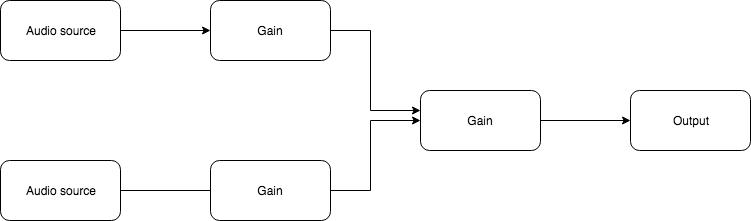
\includegraphics[scale=0.35]{img/Routing-audio-nodes-01-two-oscillators.png}
\end{figure}
\begin{itemize}
\item The gain node can be used to split and combine input sources.
\item Gain nodes facilitate independent volume control of the audio sources.
\item Gain nodes are used as virtual mixing channels.
\end{itemize}
\end{frame}
%
%
\begin{frame}
\frametitle{Modification Nodes || Effects Nodes}
\begin{itemize}
\item There exist a number of effects nodes in Web Audio (panning, EQ, delay...).
\item It is possible to combine different or similar nodes (e.g. multiple effects).
\end{itemize}
\end{frame}
%
\begin{frame}
\frametitle{How can the effects nodes be incorporated in the node graph?}
   \begin{figure}
	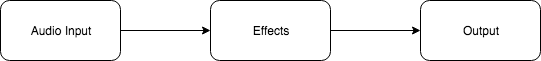
\includegraphics[scale=0.35]{img/Routing-audio-nodes-02-low-pass-filter.png}
\end{figure}
\begin{enumerate}
\item Invoke the method to create the node e.g. \textrm{AudioContext.createGain()}.
\item Connect the object in the signal chain.
\item Modify the properties and methods of the effects node.
\end{enumerate}
\end{frame}
%
\begin{frame}
\frametitle{Some of the Effects Available}
\begin{itemize}
\item \textrm{GainNode}: Volume change.
\item \textrm{StereoPannerNode}: 2D panning.
\item \textrm{BiquadFilterNode}: EQ filter.
\item \textrm{DelayNode}: Audible delay.
\item \textrm{ConvolverNode}: Convolution reverberation.
\item \textrm{DynamicsCompressorNode}: Dynamic range compression.
\end{itemize}
%\vspace{10 mm}
%\centerline{\textrm{setValueAtTime(arg1,arg2)}}
%\centerline{\textrm{exponentialRampToValueAtTime(arg1,arg2)}}
%\centerline{\textrm{linearRampToValueAtTime(arg1,arg2)}}
%\centerline{\textrm{setTargetAtTime(arg1,arg2,arg3)}}
%\centerline{\textrm{setValueCurveAtTime(arg1,arg2,arg3)}}
\end{frame}
%
\begin{frame}
\frametitle{GainNode}
The \textrm{GainNode} changes the volume. Gain nodes are also used as virtual mixing channels that can be connected in parallel or in series.\\
\vspace{10 mm}
\centerline{\textrm{AudioContext.createGain();}}
\vspace{2 mm}
\centerline{\textrm{GainNode.gain // range: 0--1}}
\vspace{10 mm}
\center{\tiny{\url{https://developer.mozilla.org/en-US/docs/Web/API/GainNode}}}
\end{frame}
%
\begin{frame}
\frametitle{StereoPannerNode}
The \textrm{StereoPannerNode} can be used to pan an audio stream left or right.\\
\vspace{10 mm}
\centerline{\textrm{AudioContext.createStereoPanner();}}
\vspace{2 mm}
\centerline{\textrm{StereoPannerNode.pan // range: -1 (L) / 1 (R)}}
\vspace{10 mm}
\center{\tiny{\url{https://developer.mozilla.org/en-US/docs/Web/API/StereoPannerNode}}}
\end{frame}
%
\begin{frame}
\frametitle{BiquadFilterNode}
The \textrm{BiquadFilterNode} represents different kinds of filters, tone control devices, and graphic equalizers.\\
\vspace{10 mm}
\centerline{\textrm{AudioContext.createBiquadFilter();}}
\vspace{2 mm}
\centerline{\textrm{BiquadFilterNode.type // options: "lowpass", "highpass", "bandpass"...}}
\vspace{10 mm}
\center{\tiny{\url{https://developer.mozilla.org/en-US/docs/Web/API/BiquadFilterNode}}}
\end{frame}
%
\begin{frame}
\frametitle{DelayNode}
The \textrm{DelayNode} causes a delay between the arrival of an input data and its propagation to the output.\\
\vspace{10 mm}
\centerline{\textrm{AudioContext.createDelay();}}
\vspace{2 mm}
\centerline{\textrm{DelayNode.delayTime // range: 0-180 seconds}}
\vspace{10 mm}
\center{\tiny{\url{https://developer.mozilla.org/en-US/docs/Web/API/DelayNode}}}
\end{frame}
%
\begin{frame}
\frametitle{ConvolverNode}
The \textrm{ConvolverNode} is often used to achieve a reverb effect.\\
\vspace{10 mm}
\centerline{\textrm{AudioContext.createConvolver();}}
\vspace{2 mm}
\centerline{\textrm{ConvolverNode.buffer}}
\vspace{10 mm}
\center{\tiny{\url{https://developer.mozilla.org/en-US/docs/Web/API/ConvolverNode}}}
\end{frame}
%
\begin{frame}
\frametitle{DynamicsCompressorNode}
The \textrm{DynamicsCompressorNode} provides a compression effect. It lowers the volume of the loudest parts of the signal in order to help prevent clipping and distortion.\\
\vspace{10 mm}
\centerline{\textrm{AudioContext.createDynamicsCompressor();}}
%\vspace{2 mm}
%\centerline{\textrm{DynamicsCompressorNode??}}
\vspace{10 mm}
\center{\tiny{\url{https://developer.mozilla.org/en-US/docs/Web/API/DynamicsCompressorNode}}}
\end{frame}
%
\begin{frame}
\frametitle{Mini-project development}
You are expected to create a mini-project that should be doable within a week. The overall aim is to get familiar with Web Audio. Here are different approaches that you can take:
\begin{itemize}
\item Develop an idea based on what we are seeing in class. Feel free to build up everyday, or change if not convinced.
\item Adapt an existing code to your needs and document what are the changes.
\item Other?
\end{itemize}
\end{frame}
%
\begin{frame}
\frametitle{Working style}
\begin{itemize}
\item Individual work but in shared rooms. You are encourage to share and discuss with your peers.
\item One-to-one talks via Zoom or personally with the instructor to catch up.
\item There will be 4 time slots during the week to work on the project. It is OK to change the topic over the course of the week. Keep a research journal.
\end{itemize}
\end{frame}
%
\begin{frame}
\frametitle{Relevant Links}
\begin{itemize}
\item Syllabus: \url{https://uio.instructure.com/courses/17406/pages/syllabus}
\item GitHub slides \& code: \url{https://github.com/axambo/audio-programming-workshop}
\end{itemize}
\end{frame}
%
%\begin{frame}
%  \frametitle{References}
%  \printbibliography
%\end{frame}
%
\end{document}
